Partie-Vorbereitung

FA-G \ref{Partie-Vorbereitung} %FA-G 126 Partie-Vorbereitung

Wahlphase

FA-G \ref{Wahlphase} %FA-G 127 Wahlphase

Ausrüstungsphase

FA-G \ref{Ausruestungsphase} %FA-G 128 Ausrüstungsphase

Startplatzverteilung der Charaktere

FA-S \ref{s-partieinit} %FA-S 8 Spiel Start und Initialisierung

Punkt verwenden

Spielzug durchführen

Bewegung durchführen

FA-G \ref{Bewegung druchfuehren} %FA-G 115 Bewegung durchführen

Drängeln

FA-G \ref{Draengeln} %FA-G 116 Drängeln

Aktion durchführen

FA-G \ref{Aktion durchfuehren} %FA-G 117 Aktion durchführen

Roulette spielen

FA-G \ref{Roulette spielen} %FA-G 119 Roulette spielen

Gadget verwenden

FA-G \ref{Gadget verwenden} %FA-G 118 Gadget verwenden
FA-G \ref{Gadgets} %FA-G 94 Gadgets

Tresor spicken

FA-G \ref{Tresor-Spicken} %FA-G 124 Tresor-Spicken

Spionieren

FA-G \ref{Spionieren} %FA-G 123 Spionieren

Charaktereigenschaft anwenden

FA-G \ref{Eigenschaften} %FA-G 73 Eigenschaften
FA-G \ref{Bang and Burn} %FA-G 90 Bang and Burn
FA-G \ref{Observation} %FA-G 93 Observation

Cocktail-Aktion durchführen

Cocktail aufnehmen

FA-G \ref{Cocktail aufnehmen} %FA-G 120 Cocktail aufnehmen
FA-G \ref{haelt Cocktail} %FA-G 75 hält Cocktail

Jemanden mit einem Cocktail übergießen

FA-G \ref{Cocktail-Guss} %FA-G 121 Cocktail-Guss

Cocktail schlürfen

FA-G \ref{Cocktail schluerfen} %FA-G 122 Cocktail schlürfen



%\begin{figure}
%  \centering
%  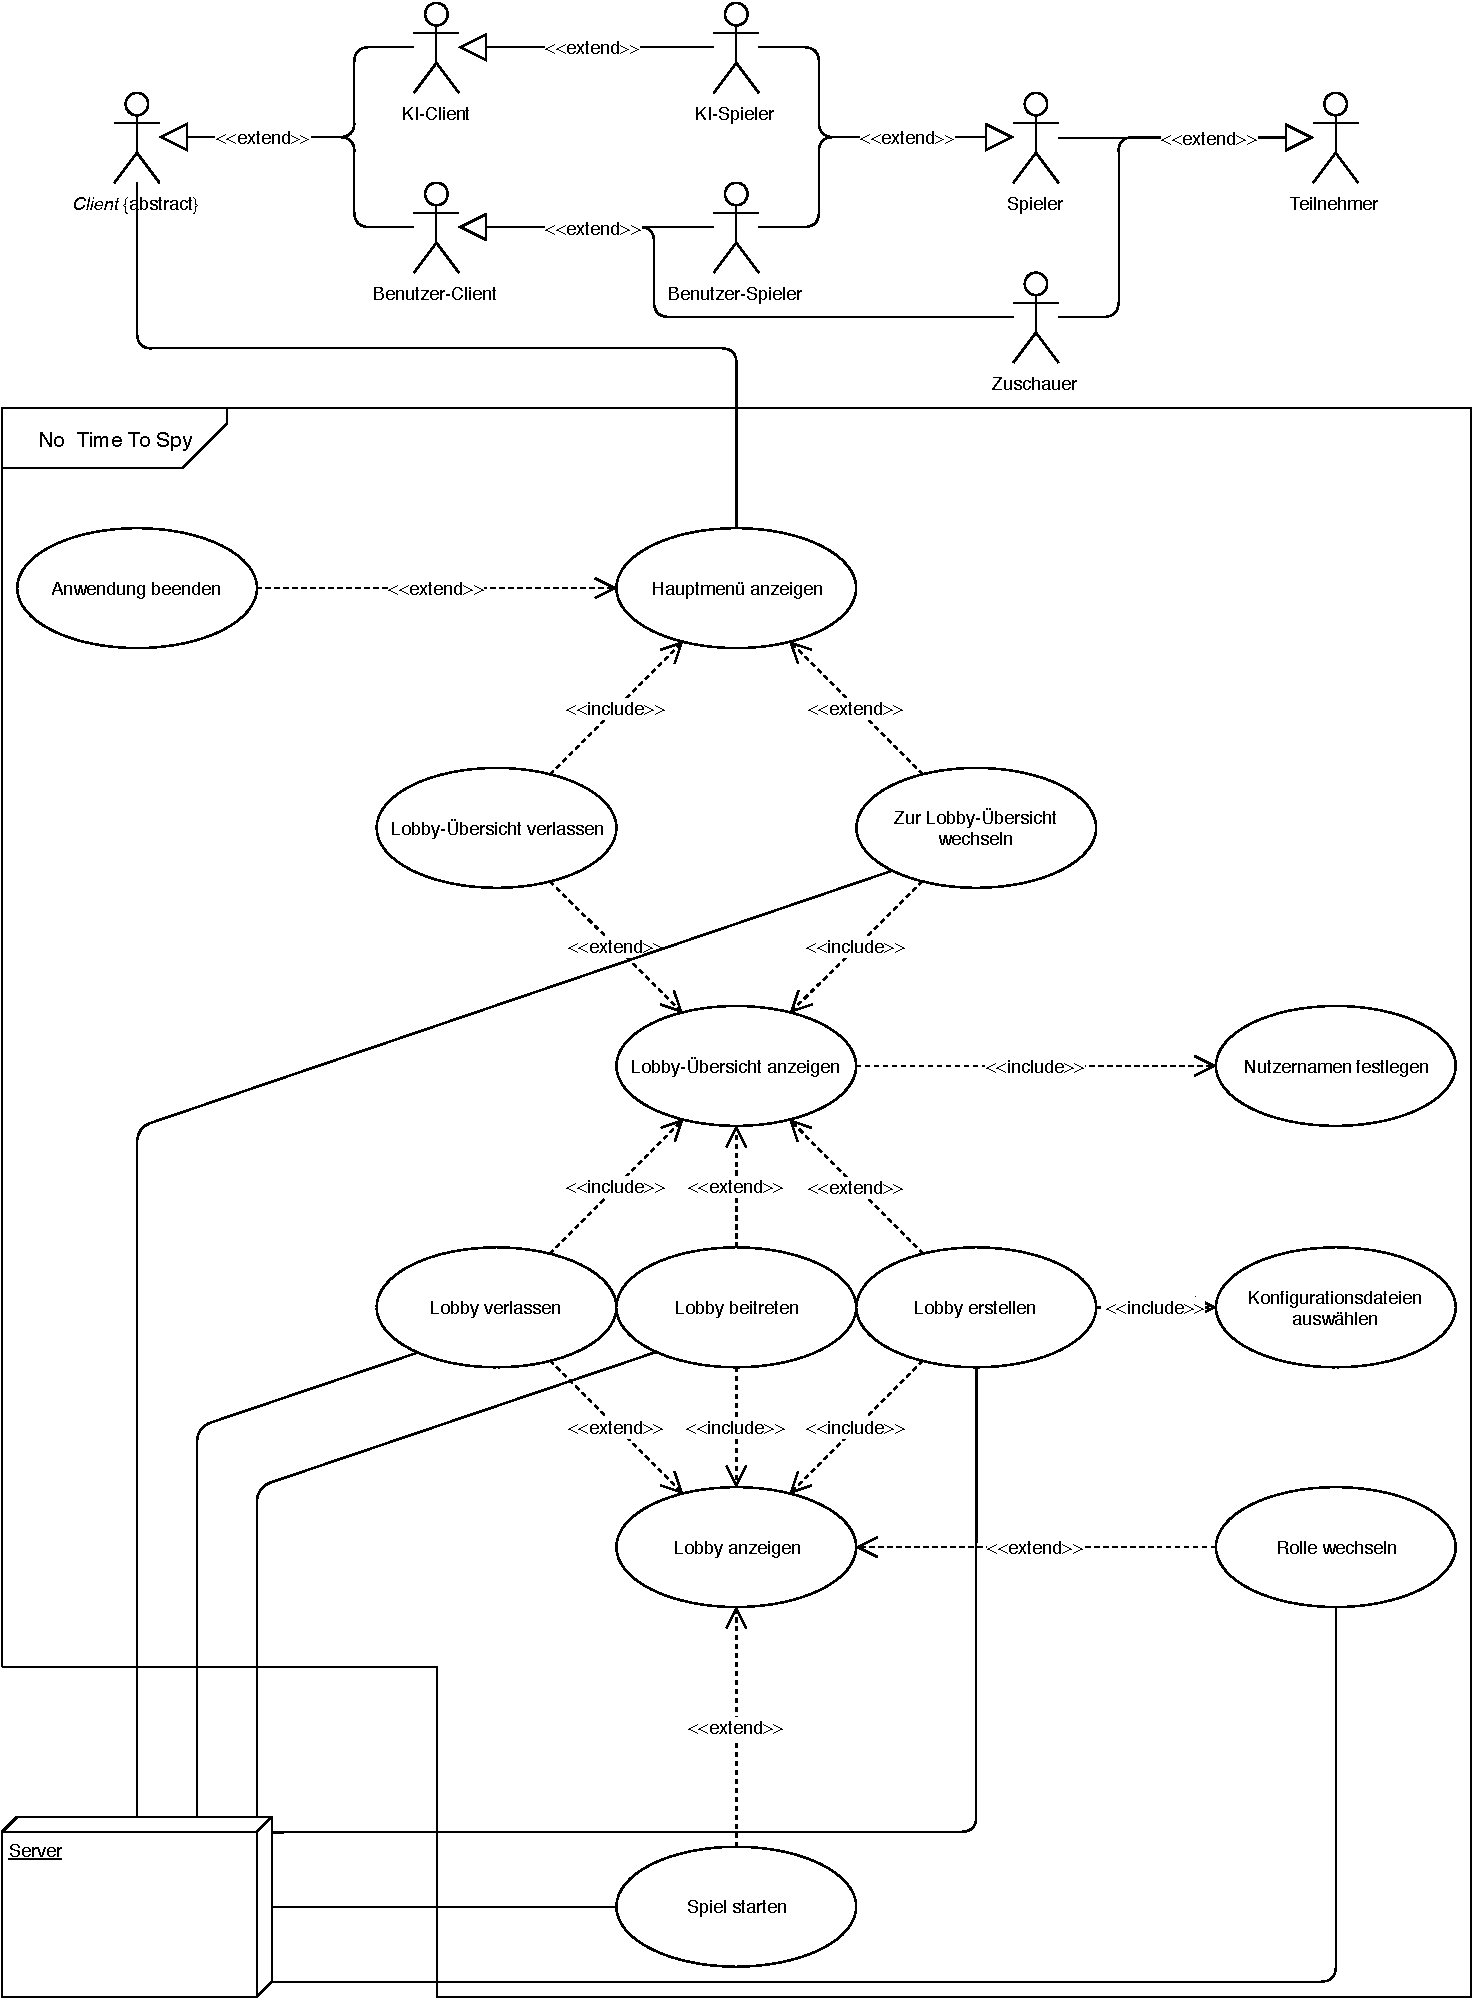
\includegraphics[width=\textwidth]{Meilenstein02/use_case_lobbymanagement.pdf}
%  \caption{Anwendungsfälle %Lobbymanagement}
%\end{figure}